
\chapter{Constellation Architecture Design
}\label{73-constellation-design-architectures}

This chapter translates the orbital mechanics framework developed in Chapter~\ref{chp:baslie_orbit_metrics} into a concrete constellation design.  Section~\ref{chp:baslie_orbit_metrics} explores the RGTO resonance design space to select the optimal seed mode and evaluates its single-satellite temporal signature over 1-day, 7-day, and 30-day horizons, including station-keeping implications; a parallel SSO seed and quantitative RGTO--SSO comparison are documented in Appendix~\ref{app:sso_orbit}.  Section~\ref{73-constellation-architectures-design} extends the single-orbit analysis to a full Walker RGTO constellation, defining the plane count and satellite phasing needed to satisfy the revisit and coverage requirements over the core study domain $\mathcal{D}_{\mathrm{core}}$.

% \begin{itemize}
% \item
%   Introduce the concept of a satellite constellation as a means to
%   improve temporal coverage.
% \item
%   Explain the fundamental constellation patterns:{ -{ -

%   \begin{itemize}
%   \item
%     \textbf{Walker Star/Delta:} Describe this as a common method for
%     achieving uniform, global coverage by distributing satellites across; =
%     multiple, evenly spaced orbital planes. Define the key parameters.
%     (T/P/F: Total satellites/Planes/Phasing).
%   \item
%     \textbf{Flower Constellations:} Briefly introduce this as a more
%     advanced concept using circular orbits to create repeating ground
%     tracks over specific regions, allowing for targeted coverage. Say that it is used as an initial configuration condition, considering only J2 perturbation, and later, other perturbations are added for a more realistic simulation in cases considering lifetime and drag. But reduce the perturbation order to simplify the simulation and reduce computational cost.
%   \item
%     \textbf{Regional Constellations:} Explain how to Repeating Ground
%     Track Orbits and the Flower Constellations Concept to optimize
%     revisit time over a region.
%   \end{itemize}
% \end{itemize}


% \chapter{Constellation Architecture Trade-Off and
% Selection}\label{chapter-8-constellation-architecture-trade-off-and-selection}

% \begin{quote}
% \textbf{Writing Guide \& Methodological Focus:}

% \begin{itemize}
% \item
%   \textbf{Objective:} To present the core original work of the thesis:
%   the simulation and analysis of{ -ifferent constellation designs.
% \item
%   \textbf{Method:} State the options, show the results for each, and
%   then compare them to make a final, justified selection.
% \item
%   \textbf{Checkpoint:} Having rigorously tested the candidate
%   architectures and chosen a final design that is clearly the most
%   efficient solution?
% \end{itemize}
% \end{quote}

% \section{Orbit Class
% Selection}\label{81-orbit-class-selection}

% % \begin{itemize}
% % \item
% %   Briefly reiterate why circular LEO is the only viable option to meet
% %   the GSD requirement, referencing the analysis in Chapter 7.
% % \end{itemize}

% As analyzed in Chapter \ref{72-earth_orbservation_orbit_candidates}, due to the mission constraints evaluated during this work development, only two types of orbits are considered for the constellation design, the Repeating Ground Track Orbits (RGTO) and the Sun-Synchronous Orbits (SSO). This section will focus on a brief comparison between RGTO Vs SSO orbits during the propagation of it's orbits for one day.
% The state vectors to chose the candidate which decreases the number of satlelites and improve the




% \section{Candidate Constellation
% Configurations}\label{82-candidate-constellation-configurations}

% \begin{itemize}
% \item
%   Formally define the architectures you will test, specifying the design
%   parameters you will vary.

%   \begin{itemize}
%   \item
%     \textbf{Architecture A (Walker Delta):} Test various T/P/F
%     combinations for this baseline global coverage model.
%   \item
%     \textbf{Architecture B (Repeating Ground Track Orbits Optimized
%     Inclined Orbits):} Test constellations with inclinations
%     specifically chosen to maximize passes over
%     Portugal\textquotesingle s latitude, taking advantage of
%     Earth\textquotesingle s gravitational perturbations.
%   \item
%     \textbf{Architecture C (Sun-Synchronous Phased Orbits):} Test a
%     constellation in a common SSO plane to evaluate performance for a
%     specific observation time.
%   \item
%     \textbf{Architecture D (Tip-Cue, Ra--Sekhmet Framework):} \textit{[Note: Introduce the mythological "Tip and Cue" naming here. High-Obs (Ra) $\rightarrow$ Low-Act (Sekhmet).]} Test a hybrid layer approach where a high-altitude asset cues the LEO fleet.
%   \end{itemize}
% \end{itemize}

% \section{Performance Simulation and
% Results}\label{83-performance-simulation-and-results}

% \begin{itemize}
% \item
%   Present the outputs of the simulations clearly.
% \item
%   For each architecture, show how the Key Parameters Metrics (KPMs).
% \item
%   (maximum work Focus)Use maps to visualize coverage statistics over Portugal for the most
%   promising configurations.
% \end{itemize}

\section{Mission Modeling And Analysis Methodological Workflow}
\label{sec:mission_modeling_workflow}

Before deriving the orbit selection metrics that follow, this section outlines the simulation and analysis pipeline from which all quantitative results in this chapter and subsequent chapters are produced.  The workflow, illustrated in Fig.~\ref{fig:mission_modeling_workflow}, chains orbit computation, high-fidelity propagation, and observation-geometry evaluation into a single reproducible process; each subsequent section applies one or more stages of this pipeline to progressively build the constellation design.

\begin{figure}[H]
    \centering
    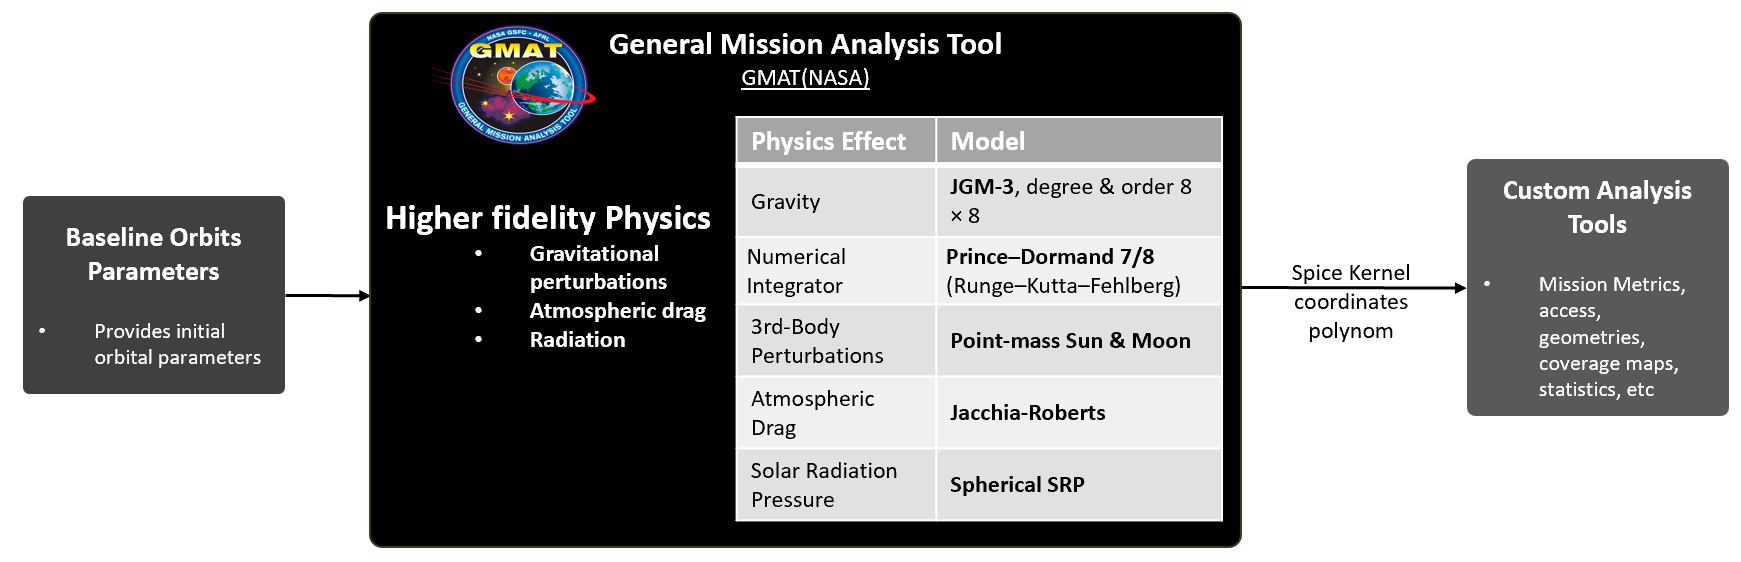
\includegraphics[width=1\linewidth]{images/mission_modeling_workflow.png}
    \caption{\footnotesize{Mission modeling and analysis workflow.  Baseline orbit parameters (Keplerian elements from the RGTO resonance analysis) are propagated in GMAT with high-fidelity physics (JGM-3 $8\times8$ gravity, Jacchia--Roberts drag, SRP, Moon/Sun perturbations).  The resulting SPICE ephemeris files are then ingested by the custom Python analysis tools to compute observation-link geometry, coverage maps, and performance statistics.}}
    \label{fig:mission_modeling_workflow}
\end{figure}

The pipeline, implemented in \texttt{Python}, comprises three stages:

\begin{enumerate}[label=\textbf{Stage~\arabic*.}, leftmargin=*, itemsep=4pt]
    \item \emph{Analytical orbit computation.}  A custom \texttt{RTGOrbit} class uses \texttt{Astropy} physical constants and \texttt{SciPy} root-finding to solve the $J_2$-perturbed resonance condition, yielding the initial Keplerian elements for each candidate orbit.

    \item \emph{High-fidelity propagation.}  The elements are imported into NASA's General Mission Analysis Tool (GMAT), which propagates the 12U~CubeSat with a Prince--Dormand~7(8) integrator, the JGM-3 $8\times8$ gravity field, Jacchia--Roberts atmospheric drag, solar radiation pressure, Sun and Moon point-mass perturbations, and relativistic corrections, using the spacecraft parameters in Table~\ref{tab:cubesat_params}.  GMAT exports the ephemerides as SPICE Binary~SPK (\texttt{.bsp}) kernels.

    \item \emph{Observation-geometry analysis.}  A custom framework loads the SPK kernels via \texttt{SpiceyPy}, transforms spacecraft states through GCRS/ITRS frames (\texttt{Astropy} \texttt{SkyCoord}), and evaluates visibility over a latitude--longitude ground grid at a fixed sampling step of $\Delta t = 10$\,s.  Each grid point undergoes a $\mathcal{F}_{J2000} \!\to\! \mathcal{F}_{SEZ}$ coordinate transformation followed by the elevation and off-nadir angle tests of the observation-link condition (Eq.~\eqref{eq:observation_link_condition}).
\end{enumerate}

\begin{table}[H]
    \centering
    \caption{\footnotesize{12U CubeSat physical parameters used in the GMAT propagation model.}}
    \label{tab:cubesat_params}
    \footnotesize
    \begin{tabular}{lcc}
        \hline
        \textbf{Parameter} & \textbf{Value} & \textbf{Unit} \\
        \hline
        Dry mass              & 18   & kg          \\
        Drag coefficient $C_d$ & 2.2  & --          \\
        Reflectivity coefficient $C_r$ & 1.3  & --  \\
        Drag area             & 0.1  & m$^{2}$     \\
        SRP area              & 0.5  & m$^{2}$     \\
        \hline
    \end{tabular}
\end{table}

The ground grid used throughout this work comprises up to $120 \times 360 = 43\,200$~points, and the GMAT ephemerides are sampled at $\Delta t = 10$\,s, yielding $N_t = 8\,640$ time steps per satellite per day.  For $N_{\mathrm{sat}=15}$ satellites the third stage must therefore evaluate
\begin{equation}
    N_{\mathrm{eval}} = N_{\mathrm{sat}} \times N_{\mathrm{grid}} \times N_t = 15 \times 43\,200 \times 8\,640 \approx 5.60 \times 10^{9} \;\text{visibility checks per day,}
    \label{eq:visibility_eval_count}
\end{equation}
visibility checks per day of propagation, each involving a coordinate transformation and the observation-link tests of Eq.~\eqref{eq:observation_link_condition}; scaling to multi-day,  monthly, annually horizons increases the workload proportionally.  Designing, implementing, and optimising this computational pipeline to handle such volumes constituted the main engineering challenge of this thesis, spanning more than one year of iterative development.  To manage the computational load the framework employs CPU-level parallelism (\texttt{ProcessPoolExecutor}, batching target points across all available cores) and optionally offloads the vectorised visibility kernel to GPU via \texttt{CuPy} (NVIDIA CUDA), reducing a single global coverage map from the order of days on a single core to several hours with multiprocessing, or to a few minutes when the GPU path is used\footnote{All simulations reported in this thesis were executed on a workstation equipped with an Intel Core i9-13900KF processor (24~cores / 32~threads, up to 5.8\,GHz), 128\,GB DDR5 RAM, and an NVIDIA GeForce RTX~4070 GPU (12\,GB GDDR6X).}.  A more detailed description of this computational framework is left for future work.




\section{Baseline Orbits Metrics Comparison}
\label{chp:baslie_orbit_metrics}

The earth observation orbit candidates were defined in Chapter~\ref{72-earth_orbservation_orbit_candidates}, where the Repeating Ground Track Orbit (RGTO) was identified as the primary orbit family for this mission.  This section presents the RGTO seed orbit metrics---resonance space, altitude--inclination selection, and single-satellite temporal signature---that drive the constellation sizing.  A parallel Sun-Synchronous Orbit (SSO) seed and the quantitative RGTO--SSO comparison are documented in Appendix~\ref{sct-SSO_seed}.

\subsubsection{RGTO Resonance Space at Coimbra: Selecting the optimal seed orbit}
\label{sec:rgto_resonance_space_coimbra}

Varying the free parameters $(N_P,\, N_D,\, i)$ in $\vec{A}_{k,\mathrm{RGTO}}$ (Eq.~\eqref{eq:rgto_element_vector}) while holding $e \approx 0$ generates a family of resonance conditions in the altitude--inclination plane.  Each point on these curves satisfies the convergence criterion of Eq.~\eqref{eq:rgto_sma_iteration}, i.e.\ the sub-satellite ground track closes after exactly $N_D$ sidereal days.  Figure~\ref{fig:RGTO_ressonantSpace} maps this design space for repeat-cycle durations $N_D = 1$ through $6$\,days.  Shorter repeat cycles confine the feasible altitudes to a narrower inclination range, which is desirable because it maximises the daily revisit rate over a given target latitude.

The analysis is now restricted to the single-day repeat case ($N_D = 1$), which minimises the revisit period to approximately one sidereal day ($T_r \approx 0.98$\,d).  Applying the constraint $i = \phi_{\text{lat}} = 40.2^{\circ}$ (Coimbra, Table~\ref{tab:pt_coords}) yields a discrete set of candidate altitudes---one per integer $N_P$---shown in Fig.~\ref{fig:RGTO_1day_resonance}.  Modes $N_P = 12$--$13$ fall in the MEO range ($h > 800$\,km), where the larger Earth-disc distance degrades the Ground Sample Distance (GSD).  Mode $N_P = 16$ descends into the VLEO regime ($h < 450$\,km), where atmospheric drag severely limits mission lifetime without continuous station-keeping.  The mode $\tau = 15/1$ at $h \approx 488$\,km occupies the lower Earth Observation band, offering a favourable trade-off between spatial resolution, mission lifetime, and temporal coverage ($T_S \approx 5652$\,s per revolution).

\begin{figure}
    \centering
    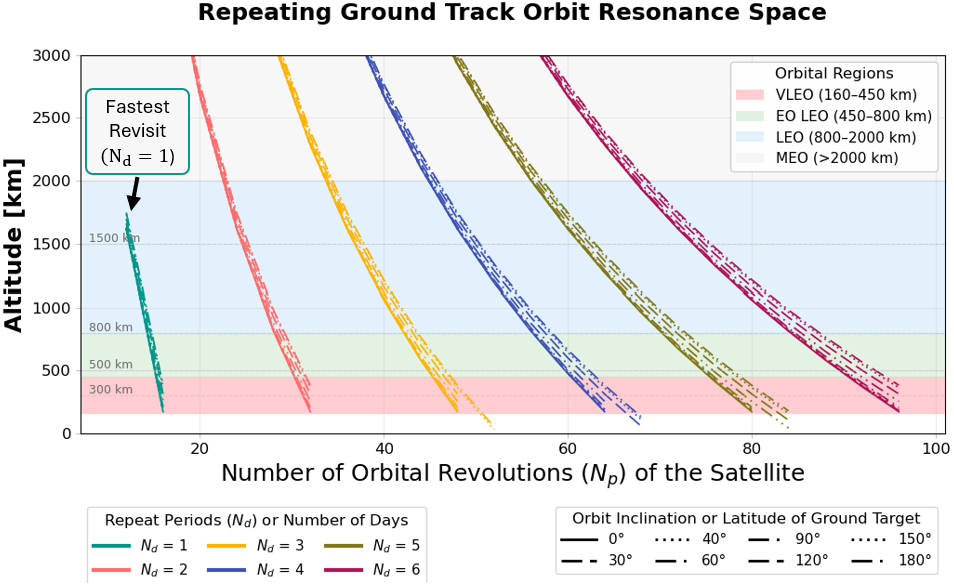
\includegraphics[width=0.92\linewidth]{images/RGTO_ressonantSpace.png}
    \caption{\footnotesize{RGTO resonance design space: orbital altitude $h$ as a function of inclination $i$ for repeat-cycle durations $N_D = 1$ through $6$\,days.  Each curve corresponds to a fixed number of revolutions per cycle~$N_P$; increasing $N_P$ lowers the orbital altitude.  Shorter repeat cycles concentrate the feasible altitude--inclination pairs into a narrower band, enabling faster ground-track revisit.}}
    \label{fig:RGTO_ressonantSpace}
\end{figure}

\begin{figure}
    \centering
    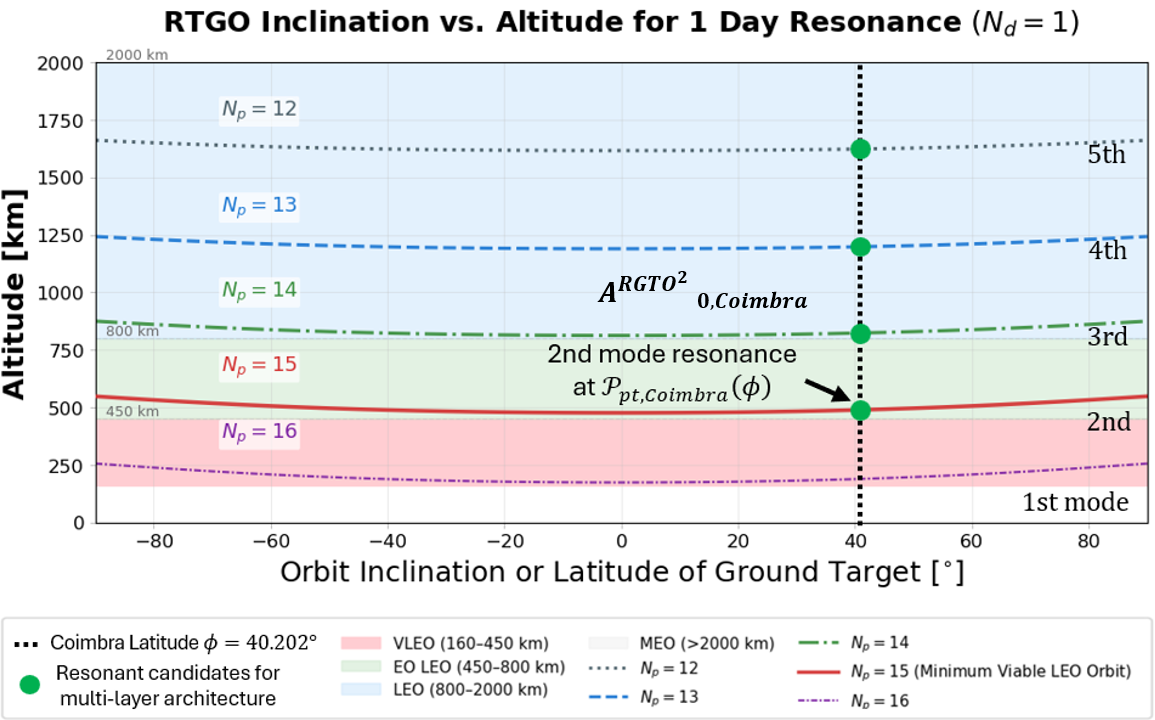
\includegraphics[width=0.92\linewidth]{images/RGTO_1day_resonance.png}
    \caption{\footnotesize{Detail of the $N_D = 1$ resonance space showing altitude versus inclination for $N_P \in [12,\,16]$.  The vertical line at $i = \phi_{\text{lat}} = 40.2^{\circ}$ (Coimbra latitude, Table~\ref{tab:pt_coords}) intersects the resonance curves, defining the five candidate modes listed in Table~\ref{tab:rgto_parameters_coimbra}.  Shaded altitude bands indicate the Very Low Earth Orbit (VLEO, $h < 450$\,km), Earth Observation (EO, $450$--$800$\,km), and Medium Earth Orbit (MEO, $h > 800$\,km) regimes.  The selected mode $\tau = 15/1$ ($h \approx 488$\,km) lies at the lower bound of the EO band.}}
    \label{fig:RGTO_1day_resonance}
\end{figure}



for the constellation architecture: the $\tau = 15/1$ mode at $h \approx 488$\,km.  This configuration provides the best trade-off between fast revisit (one sidereal day), high spatial resolution (lower EO band), and viable mission lifetime (manageable atmospheric drag).  The complete set of derived orbital parameters for all five candidate modes is presented in Sec.~\ref{sec:rgto_parametric_results}.

From this analysis we create a nomenclature to define the orbital element vector of a RGTO of mode $n$ with index k resonating with an Earth point target P as $\vec{\mathbf{A}}^{\,\mathrm{RGTO}^{\, n}}{}_{k,\,\mathrm{P}}$, where $n$ is the integer number modes of this resonant orbit, with n=1 the closest to the planet surface.

Figure~\ref{fig:RGTO_1day_resonance} show the optimal seed case is modeled by the orbital element vector k=0 describing a RGTO of second mode at Coimbra defined as:
\begin{equation}
  \vec{\mathbf{A}}^{\,\mathrm{RGTO}^{\,2}}{}_{0,\,\mathrm{Coimbra}} = \bigl[15/1,\; 0.001,\; 40.2033^{\circ},\; 0^{\circ},\; 0^{\circ},\; 0^{\circ} ,\; 0s\bigr]^{T}
\label{eq:RGTO_2_coimbra}
\end{equation}
The complete set of derived orbital parameters for all five candidate modes is presented in Sec.~\ref{sec:rgto_parametric_results}.

\subsubsection{RGTO Parametric Results at Coimbra}
\label{sec:rgto_parametric_results}

Table~\ref{tab:rgto_parameters_coimbra} summarises the derived orbital parameters for five candidate resonance orbits modes ($\tau = 12/1$ through $16/1$) evaluated at the Coimbra target latitude, table \ref{tab:pt_coords}, \reqRef{R14}.  All modes share the common initial conditions of been near circular orbit at the same plane and epoch.

\begin{table}[H]
\centering
\caption{\footnotesize{RGTO seed orbit parameters for five resonance modes at Coimbra ($\phi_{\text{lat}} \approx 40.20329^{\circ}$\,N).  Common conditions: $e = 0.001$, $\omega = 0^{\circ}$, $\Omega = 0^{\circ}$, $M = 0^{\circ}$.  The semi-major axis $a$ is obtained via the iterative scheme of Eq.~\eqref{eq:rgto_sma_iteration}; perturbation rates follow from the $J_2$ secular theory (Sec.~\ref{sec:perturbed_orbital_elements}).}}
\label{tab:rgto_parameters_coimbra}
\smallskip
\footnotesize
\setlength{\tabcolsep}{4pt}
\begin{tabular}{c l r r r r r r r r r}
\toprule
$n$
  & $\tau\;(N_P\!/N_D)$
  & $a$ [km]
  & $h$ [km]
  & $i$ [$^{\circ}$]
  & $T_S$ [s]
  & $T_G$ [s]
  & $T_r$ [d]
  & $\dot{\Omega}$ [rad\,s$^{-1}$]
  & $\dot{\omega}$ [rad\,s$^{-1}$]
  & $\dot{M}$ [rad\,s$^{-1}$] \\
\midrule
5 & 12/1 & 8000.90  & 1622.80 & 40.20329  & 7112  & 85\,350 & 0.9879  & $-6.95{\times}10^{-7}$ & $8.72{\times}10^{-7}$ & $8.83{\times}10^{-4}$ \\
4 & 13/1 & 7575.91  & 1197.81 & 40.220329  & 6552  & 85\,180 & 0.9859  & $-8.42{\times}10^{-7}$ & $1.06{\times}10^{-6}$ & $9.58{\times}10^{-4}$ \\
3 & 14/1 & 7200.84  & 822.74  & 40.20329  & 6071  & 84\,990 & 0.9837  & $-1.01{\times}10^{-6}$ & $1.26{\times}10^{-6}$ & $1.03{\times}10^{-3}$ \\
\rowcolor{green!15} {\bfseries 2} & {\bfseries 15/1$^{\dagger}$} & {\bfseries 6866.64}  & {\bfseries 488.54}  & {\bfseries 40.20329}  & {\bfseries 5652}  & {\bfseries 84\,780} & {\bfseries 0.9813}  & {\bfseries $-1.19{\times}10^{-6}$} & {\bfseries $1.49{\times}10^{-6}$} & {\bfseries $1.11{\times}10^{-3}$} \\
1 & 16/1 & 6566.35  & 188.25  & 40.20329  & 5285  & 84\,550 & 0.9786  & $-1.39{\times}10^{-6}$ & $1.74{\times}10^{-6}$ & $1.19{\times}10^{-3}$ \\
\bottomrule
\end{tabular}
\\[2pt]
{\footnotesize \parbox{0.97\linewidth}{$^{\dagger}$ Selected baseline RGTO seed candidate: this mode provides the best trade-off for fast revisit, maximum coverage over the core study domain $\mathcal{D}_{\mathrm{core}}$, and viable mission lifetime.}}
\label{tab:rgto_family_coimbra}
\end{table}

To validate the RGTO selection, the seed orbit was benchmarked against a Sun-Synchronous Orbit (SSO) baseline derived from SpaceX Transporter rideshare injection parameters ($a = 6904$\,km, $h \approx 525.9$\,km, $i_{\mathrm{SSO}} = 97.50^{\circ}$).  The full SSO seed derivation and the 7-day observation-link comparison are presented in Appendix~\ref{sct-rgto_vs_sso}.  The key finding is that the near-polar SSO crosses Coimbra's latitude at a steep angle with limited permanence time, whereas the RGTO ground track aligns with the target latitude, yielding approximately 1.75 times the daily coverage rate.  Consequently, an SSO-based constellation would require roughly twice as many satellites to achieve equivalent temporal coverage, confirming the RGTO as the preferred orbit class for this mission.

\section{Constellation Architectures Design}\label{73-constellation-architectures-design}

The selected seed orbit $\vec{\mathbf{A}}^{\,\mathrm{RGTO}^{\,2}}{}_{0,\,\mathrm{Coimbra}}$ (Eq.~\eqref{eq:rgto_element_vector}) is propagated over 1-day and 7-day windows to characterise its temporal coverage signature at the Coimbra ground station before addressing the full constellation.  Figures~\ref{fig:RGTO_maps_Coimbra_One_day}--\ref{fig:RGTO_metrics_Coimbra_Seven_days} present the ground-track geometry and the associated observation-link metrics; the revisit structure derived here drives the plane and satellite-count trade-off in the sections that follow.

\subsection{Single-Satellite Temporal Signature over 1-Day}
\label{sec:seed_1day_propagation}

The seed orbit is first propagated over a single day coinciding with the peak fire reference date (August~18, \reqRef{R16}) to characterise the repeating-ground-track geometry and the observation-link signature at Coimbra.

Figure~\ref{fig:RGTO_maps_Coimbra_One_day} presents the geometrical view.  The ground-track plot~(B) confirms the resonance condition: the sub-satellite trace overlaps itself precisely over the 1-day window.  At the latitude of Coimbra, the observation-link access boundary is marked by the blue dashed line, corresponding to the minimum elevation mask $\varepsilon_{\min} = 15^{\circ}$.  The sky plot~(A) displays the same passes in a polar azimuth--elevation diagram (elevation $0^{\circ}$ at the rim, $90^{\circ}$~=~zenith at the centre).  Four passes cross the Coimbra sky within a single day; they span approximately from 12:46 to 17:50~local time, and the closest nadir approach---the greenish-yellow trajectory---occurs near 15:00\,LT, coinciding with the peak fire observation window \reqRef{R35}.

The quantitative observation-link metrics are detailed in Fig.~\ref{fig:RGTO_metrics_Coimbra_One_day}.  Plot~(A) shows the visibility timeline: four successive passes satisfy the observation-link condition (Eq.~\ref{eq:observation_link_condition}), i.e.\ the logical conjunction of the ground-segment access $\varepsilon \geq \varepsilon_{\min} = 15^{\circ}$ and the space-segment access $\eta \leq \eta_{\max} = 65^{\circ}$.  The inter-revisit gap between consecutive passes is $t_{\mathrm{rev,RGTO}} \approx 99.23$\,min, and the four passes together form a single-day observation sequence window of $T_{\mathrm{seq,RGTO}} \approx 4$\,h\,57\,min.

Plot~(B) displays the elevation and distance profiles.  The elevation peaks vary across the four passes---from $\sim\!40^{\circ}$ for the first, through $\sim\!80^{\circ}$ and $\sim\!75^{\circ}$ for the second and third, down to $\sim\!25^{\circ}$ for the fourth---while the minimum slant distance reaches approximately 500\,km at closest approach.  All passes remain above $\varepsilon_{\min}$.

Plot~(C) presents the off-nadir angle~$\eta$ and the corresponding Ground Sample Distance on the right axis.  The off-nadir angle reaches minima of $\sim\!25^{\circ}$, $\sim\!10^{\circ}$, $\sim\!12^{\circ}$, and $\sim\!47^{\circ}$ for the four passes respectively, and the GSD remains below $6$\,m/pixel throughout, satisfying the spatial resolution requirement \reqRef{R8} under the paraxial GSD model Eq.~\ref{eq:gsd}.

The key outcome of this 1-day analysis is the identification of the seed temporal pattern: four passes clustered within a $\sim$5-hour window, separated by $\sim$99-minute gaps, leaving the remaining $\sim$19~hours of the day unobserved.  To extend coverage throughout the full day, this pattern can be replicated by introducing additional satellites in the same orbital plane, phased by a true-anomaly shift~$\Delta\nu$, such that their observation sequences fill the inter-sequence gaps.  Once a single plane achieves the target intra-plane revisit, the plane itself is replicated at different rotations around the reference orthogonal axis to map different RAAN values to cover the full sidereal day.  This two-level approach of populating a plane, then distributing planes, is developed in Section~\ref{sec:constellation_plane1}.

\begin{figure}
    \centering
    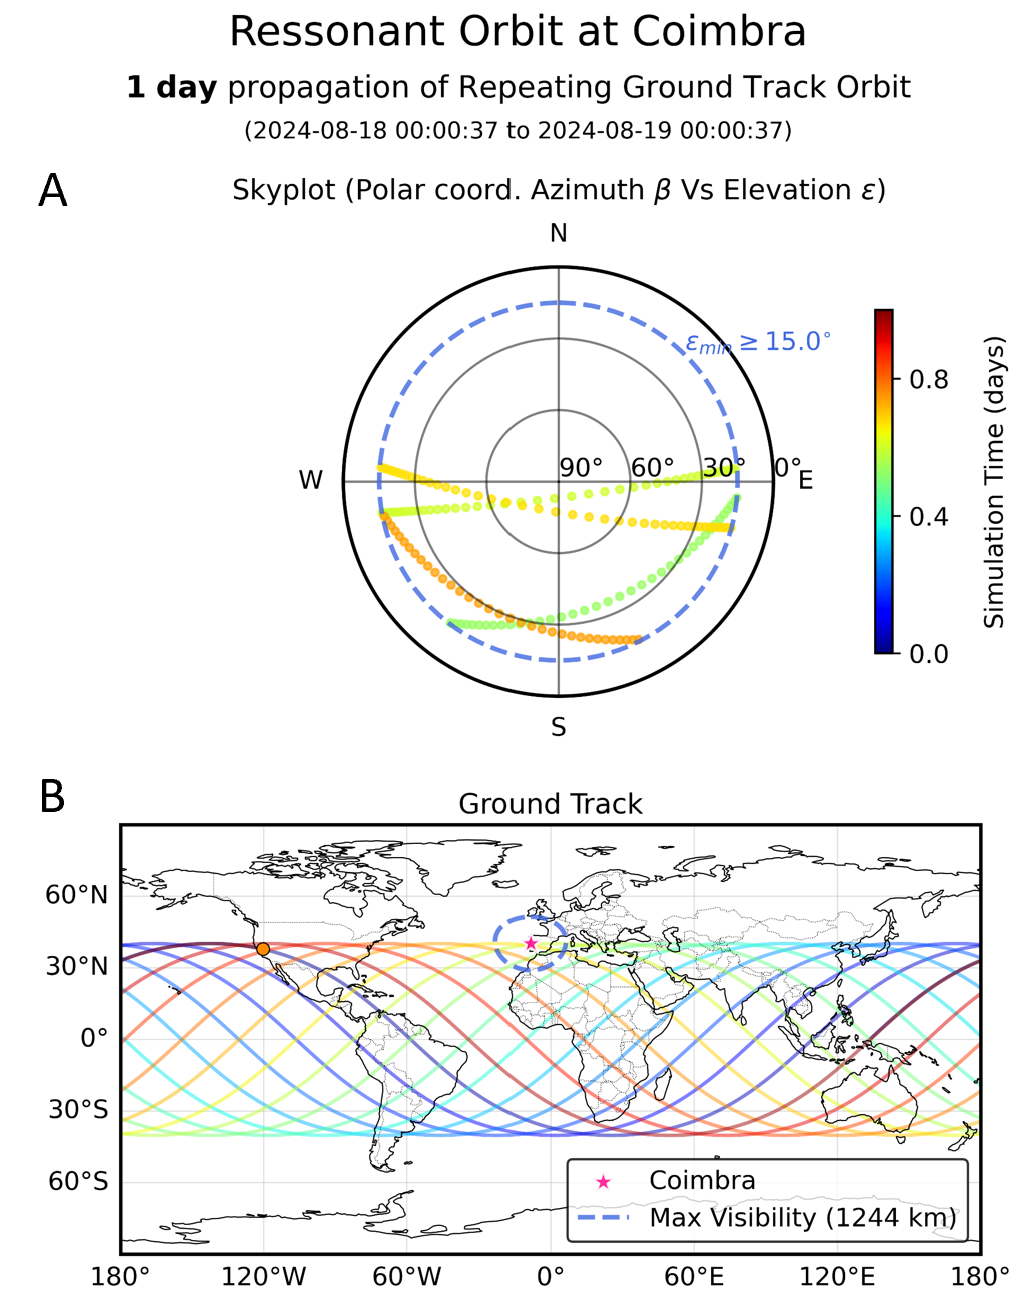
\includegraphics[width=0.9\linewidth]{images/RGTO_maps_Coimbra_One_day.png}
    \caption{1-day RGTO seed propagation over Coimbra ($\tau = 15/1$, $h \approx 488$\,km, $i = 40.2^{\circ}$, 2024 August~18) verifying resonance condition pattern.  \textbf{(A)}~Azimuth--elevation sky plot; four passes cross the sky between $\sim$12:46 and $\sim$17:50\,LT, with the near-nadir pass at $\sim$15:00\,LT.  \textbf{(B)}~Ground-track map; the blue dashed line marks the $\varepsilon_{\min} = 15^{\circ}$ observation-link access boundary.}
    \label{fig:RGTO_maps_Coimbra_One_day}
\end{figure}

\begin{figure}
    \centering
    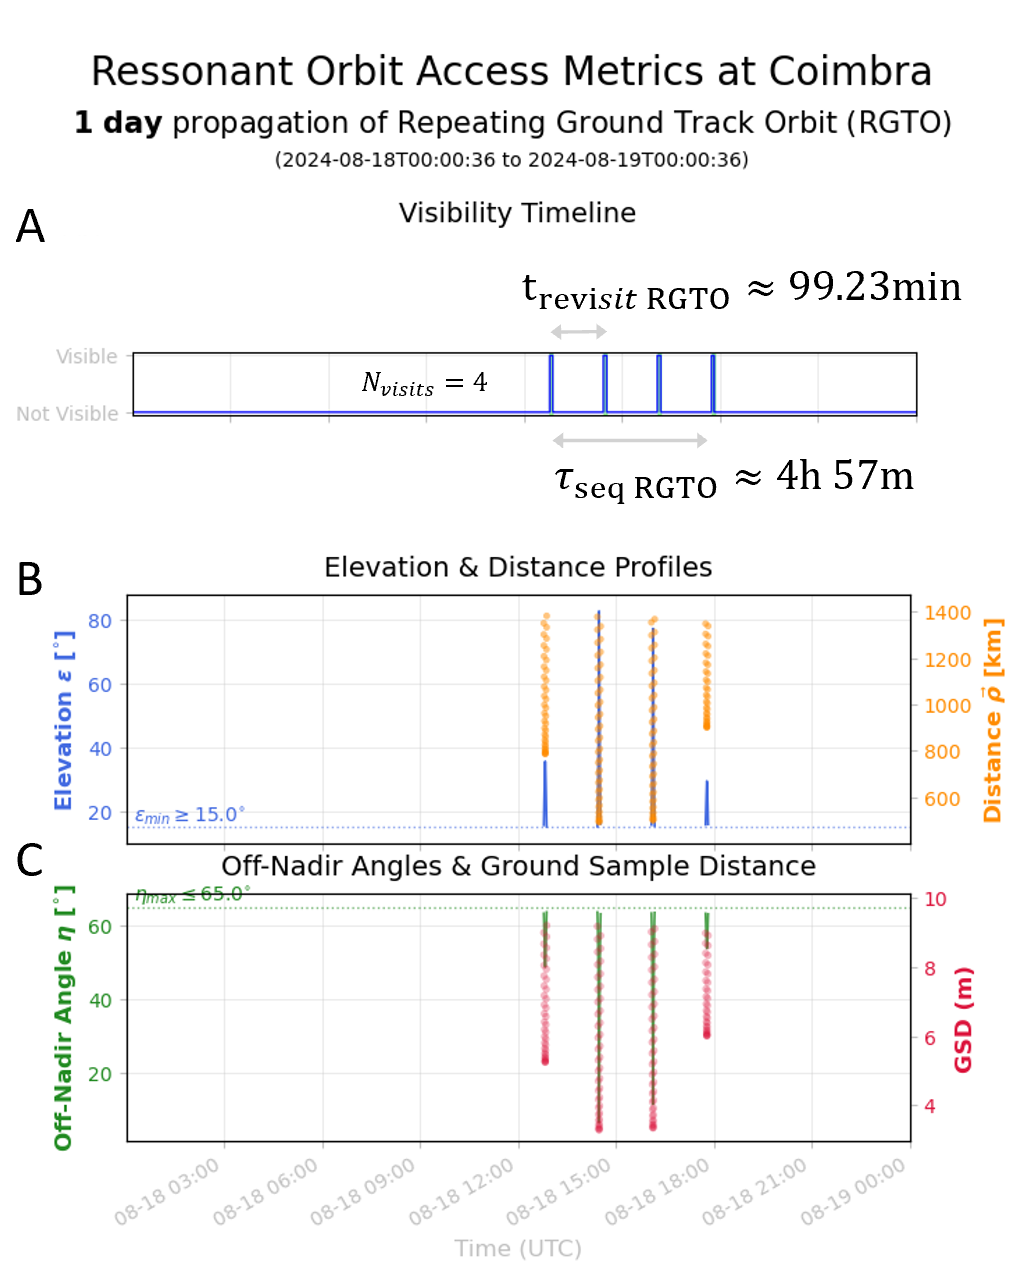
\includegraphics[width=1\linewidth]{images/RGTO_metrics_Coimbra_One_day.png}
    \caption{Observation-link metrics for the 1-day RGTO propagation at Coimbra.  \textbf{(A)}~Visibility timeline: four passes with inter-revisit gap $t_{\mathrm{rev,RGTO}} \approx 99.23$\,min forming a sequence window $T_{\mathrm{seq,RGTO}} \approx 4$\,h\,57\,min.  \textbf{(B)}~Elevation and slant-distance profiles.  \textbf{(C)}~Off-nadir angle~$\eta$ and GSD (right axis); GSD\,$< 6$\,m/pixel for all passes.}
    \label{fig:RGTO_metrics_Coimbra_One_day}
\end{figure}


\subsection{Single-Satellite Temporal Signature over 7-Days}
\label{sec:seed_7day_propagation}

The same seed orbit is propagated over a 7-day window to verify the persistence of the resonance pattern under atmospheric drag and $J_{8\times8}$ gravitational perturbations.  The ground-track and sky-plot maps for this period (Appendix~\ref{sec:appendix_7day_maps}, Fig.~\ref{fig:RGTO_maps_Coimbra_Seven_days}) confirm that the sub-satellite trace overlaps the 1-day pattern (Fig.~\ref{fig:RGTO_maps_Coimbra_One_day}) without appreciable drift, and the four-pass cluster recurs daily with consistent azimuth--elevation trajectories.

\begin{figure}
    \centering
    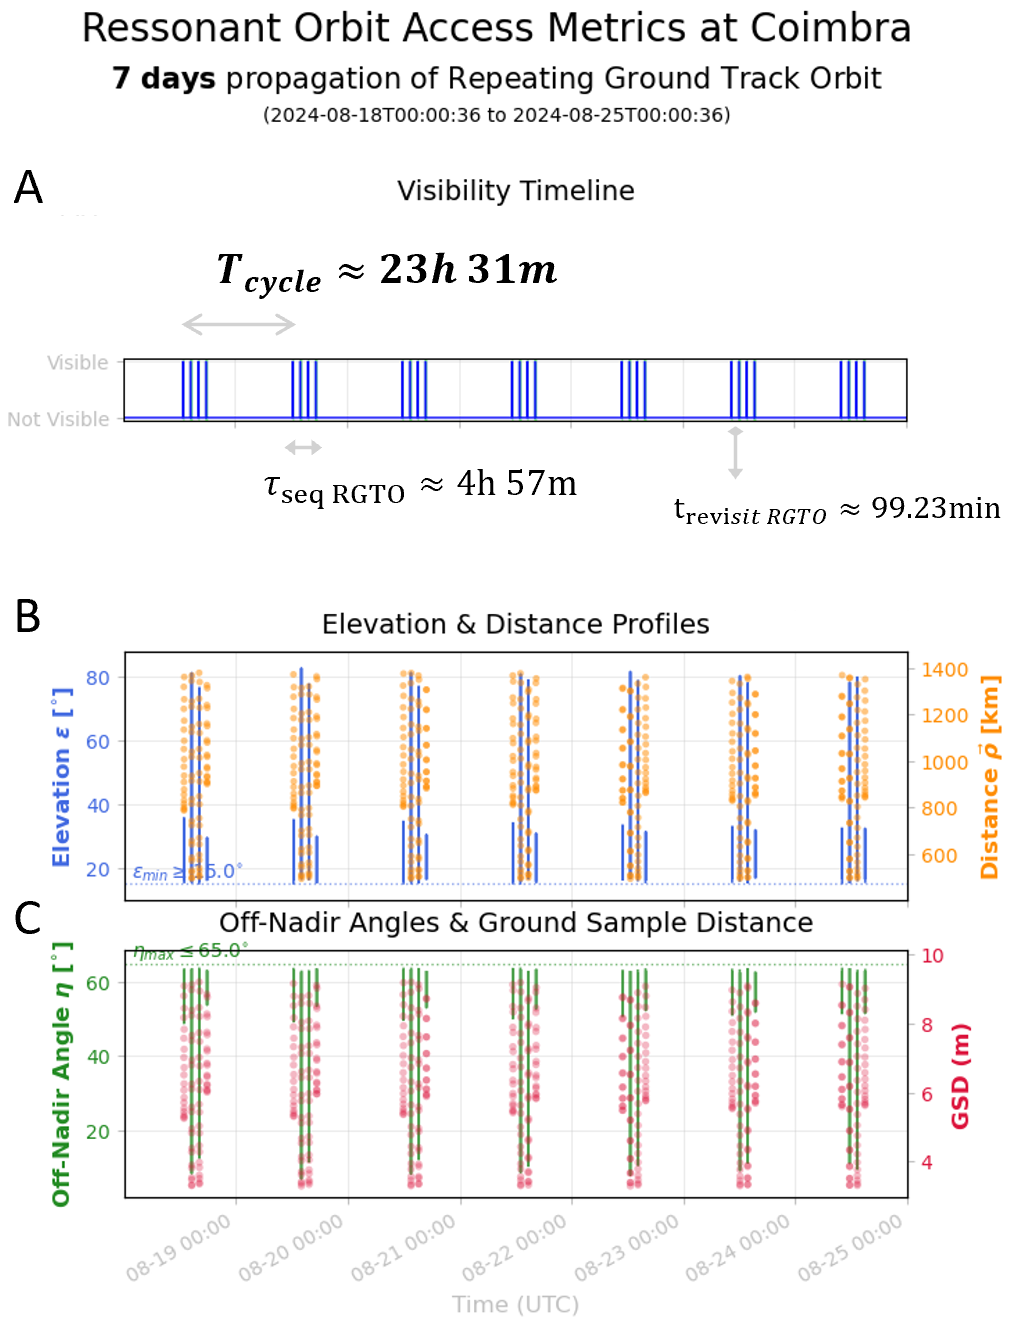
\includegraphics[width=1\linewidth]{images/RGTO_metrics_Coimbra_Seven_days.png}
    \caption{Observation-link metrics for the 7-day RGTO propagation at Coimbra.  \textbf{(A)}~Visibility timeline: the four-pass sequence repeats with $T_{\mathrm{rep,RGTO}} \approx 23$\,h\,30\,min (28~passes total).  \textbf{(B)}~Elevation and distance profiles across all passes.  \textbf{(C)}~Off-nadir angle and GSD; quality remains within the 1-day envelope.}
    \label{fig:RGTO_metrics_Coimbra_Seven_days}
\end{figure}

The observation-link metrics for the 7-day window (Fig.~\ref{fig:RGTO_metrics_Coimbra_Seven_days}) quantify this recurrence.  The visibility timeline~(A) shows the four-pass sequence repeating with a near-sidereal cycle $T_{\mathrm{rep,RGTO}} \approx 23$\,h\,30\,min, yielding 28~passes over 7~days (four per cycle).  The effective observation window per day remains $T_{\mathrm{seq,RGTO}} \approx 5$\,h, consistent with the 1-day result.  The elevation and distance profiles~(B) across all 28~passes show no degradation attributable to drag.  The off-nadir angle and GSD~(C) remain within the 1-day envelope, with GSD\,$< 6$\,m/pixel for all passes, confirming sustained optical performance.

The stable daily recurrence of the $\sim$5-hour observation window validates the design premise: the seed temporal pattern identified in the 1-day propagation is a persistent feature of the RGTO resonance, not a single-epoch artefact.  The next step (Section~\ref{sec:constellation_plane1}) exploits this periodicity by distributing additional satellites within one plane, phased by $\Delta\nu$ to overlap their observation sequences and reduce the intra-plane revisit gap, and then replicating the populated plane at different RAAN values to achieve full-day coverage satisfying the mission requirement $t_{\text{revisit}} \leq 30$\,min \reqRef{R7}.


The RGTO resonance demonstrated in the 1-day and 7-day windows relies on the orbit altitude remaining close to the design value $h \approx 488$\,km.  Atmospheric drag progressively lowers the semi-major axis, and the repeating ground-track condition degrades over time scales longer than approximately one month.  

A detailed analysis of the resonance drift---including 30-day and 1-year uncontrolled propagations, a simplified altitude-maintenance algorithm implemented in NASA GMAT, and end-of-life lifetime estimation---is presented in Appendix~\ref{app:station_keeping}.  
The key conclusions are that four station-keeping burns per year are sufficient to preserve the resonance, and the uncontrolled orbital lifetime for the assumed 12U CubeSat parameters is approximately 3.5~years, indicating that an operational satellite must possess station-keeping capability for a cost-effective service.  This analysis also confirms that the RGTO seed orbit at this altitude is stable and serves as the constellation building block for the mission design developed in the next section.

\subsection{Baseline Constellation Architecture}\label{sec:baseline_constellation_architecture}

The preceding analysis demonstrates that, across coverage, revisit-time, and GSD metrics, the RGTO seed orbit $\vec{\mathbf{A}}^{\,\mathrm{RGTO}^{\,2}}{}_{0,\,\mathrm{Coimbra}}$ outperforms the SSO candidate (Appendix~\ref{sct-rgto_vs_sso}) and is therefore selected as the constellation building block.  Each satellite is defined as
\begin{equation}
  S_{\mathrm{core},\,k} \;=\; S_k\!\left(\vec{\mathbf{A}}^{\,\mathrm{RGTO}^{\,2}}{}_{k,\,\mathrm{Coimbra}}\right),
\end{equation}
where the index $k$ distinguishes individual spacecraft regardless of their operational state.  The design question is: how should the set $\{S_{\mathrm{core},\,k}\}$ be distributed across orbital planes to maximise coverage over the core study domain $\mathcal{D}_{\mathrm{core}}$ while minimising the total satellite count $N_{\mathrm{sat}}$?  A co-planar insertion strategy is preferred because satellites sharing the same $(\Omega, i)$ can be deployed in a single launch, reducing mission cost.

The Walker-$\delta$ constellation framework \cite{walker_circular_1970} provides a systematic solution: satellites are uniformly distributed across $P$ equally spaced orbital planes with defined inter-satellite phasing (see Appendix~\ref{sec:appendix_walker_example}, Fig.~\ref{fig:constellation_walker_12_sats_3planes_ example}).  In Walker-$\delta$ notation the inclination equals the pattern parameter, $i = \delta$.  In this work a constellation is denoted $\mathcal{C}_{T/P/F}$, where $T$ is the total number of satellites, $P$ the number of planes, and $F$ the RAAN spacing between adjacent planes.  Individual spacecraft are labelled $P_jS_k$, where $j$ identifies the plane and $k$ the satellite within that plane.

\subsubsection{Defining the Constellation Seed Plane~1}
\label{sec:constellation_plane1}

The single-satellite temporal pattern established in the 1-day and 7-day propagations (Sections~\ref{sec:seed_1day_propagation}--\ref{sec:seed_7day_propagation}) shows that one RGTO satellite produces a $\sim$5-hour cluster of passes per day over Coimbra.  To improve the passes frequency, Plane $P_1$ is populated with three satellites phased uniformly in true anomaly ($\Delta\nu = 120^{\circ}$). Now the revisit time in Plane 1 $t_{\mathrm{rev,P1}}$ is defined as interval between passes of the cluster of the three satellites in P1S1, P1S2, and P1S3, reducing the previous revisit of unique satellite from 99min to  to approximately $t_{\mathrm{rev,P1}=33.4}$\,min. A detailed explanation of this process is given in the next paragraphs.

Figure~\ref{fig:temporal_res_P1S1} presents the observation-link analysis for this three-satellite plane.  Panel~(a) shows the combined observation-link condition, formed by the logical conjunction of the ground-segment access window $W_{\mathrm{ground}}$ ($\varepsilon \geq 15^{\circ}$) and the space-segment access window $W_{\mathrm{space}}$ ($\eta \leq 65^{\circ}$).  Panel~(b) displays the elevation profile: consecutive passes from $P_1S_1$, $P_1S_2$ and $P_1S_3$ overlapped to yield an intra-plane revisit of $t_{\mathrm{rev,P1}} \approx 33.4$\,min, close to the $\leq 30$\,min requirement \reqRef{R7}.  Panel~(c) shows the off-nadir angle for each pass; passes near $\eta \approx 60^{\circ}$ suffer degraded imaging quality but remain usable for data relay.

Two characteristic time windows emerge from this plane.  The \emph{effective sequence window} $T_{\mathrm{seq,eff}} \approx 297$\,min spans the passes that fully satisfy both the elevation and off-nadir criteria with comfortable margins, and when combined with other adjacent satellites passes in next orbital planes, produces a gap-free observation cluster.  The \emph{maximum sequence window} $T_{\mathrm{seq,max}} \approx 364.5$\,min extends to the outermost passes that technically meet the observation-link thresholds but are marginal---high $\eta$ near the cut-off, low $\varepsilon$ near the mask---leading to inter-plane gaps and over-constraining the sensor effective field of view.

The number of orbital planes required for full-day coverage follows from dividing the sidereal day by the chosen sequence window:
\begin{equation}
  N_P \;=\; \left\lceil \frac{1440\;\mathrm{min}}{T_{\mathrm{seq}}} \right\rceil.
\end{equation}
Using $T_{\mathrm{seq,max}}$ yields $N_P = \lceil 1440/364.5 \rceil = 4$ planes with RAAN phasing $\delta\Omega = 90^{\circ}$.  The resulting $\mathcal{C}_{12/4/90}$ constellation, however, exhibits visible coverage gaps between consecutive plane windows (see Appendix~\ref{sec:appendix_4plane_obs}, Fig.~\ref{fig:obs_links_4planes}), confirming that the marginal passes at the edges of $T_{\mathrm{seq,max}}$ do not provide reliable temporal uniformity.

Adopting $T_{\mathrm{seq,eff}}$ instead gives $N_P = \lceil 1440/297 \rceil = 5$ planes with phasing $\delta\Omega = 360^{\circ}/5 = 72^{\circ}$.  The five RAAN values, anchored to the reference $\Omega_{\mathrm{ref}} = 100^{\circ}$ (aligned with the 18~August fire-peak pass at 15:00\,LT), are $\Omega_{P1}=100^{\circ}$, $\Omega_{P2}=172^{\circ}$, $\Omega_{P3}=244^{\circ}$, $\Omega_{P4}=316^{\circ}$, $\Omega_{P5}=28^{\circ}$.  Figure~\ref{fig:obs_links_5planes} shows that this 5-plane configuration achieves continuous high-quality observation-link coverage over the full day, with $t_{\mathrm{rev}} \lesssim 33$\,min, satisfying both the temporal \reqRef{R7} and spatial \reqRef{R8} requirements.

\begin{figure}
    \centering
    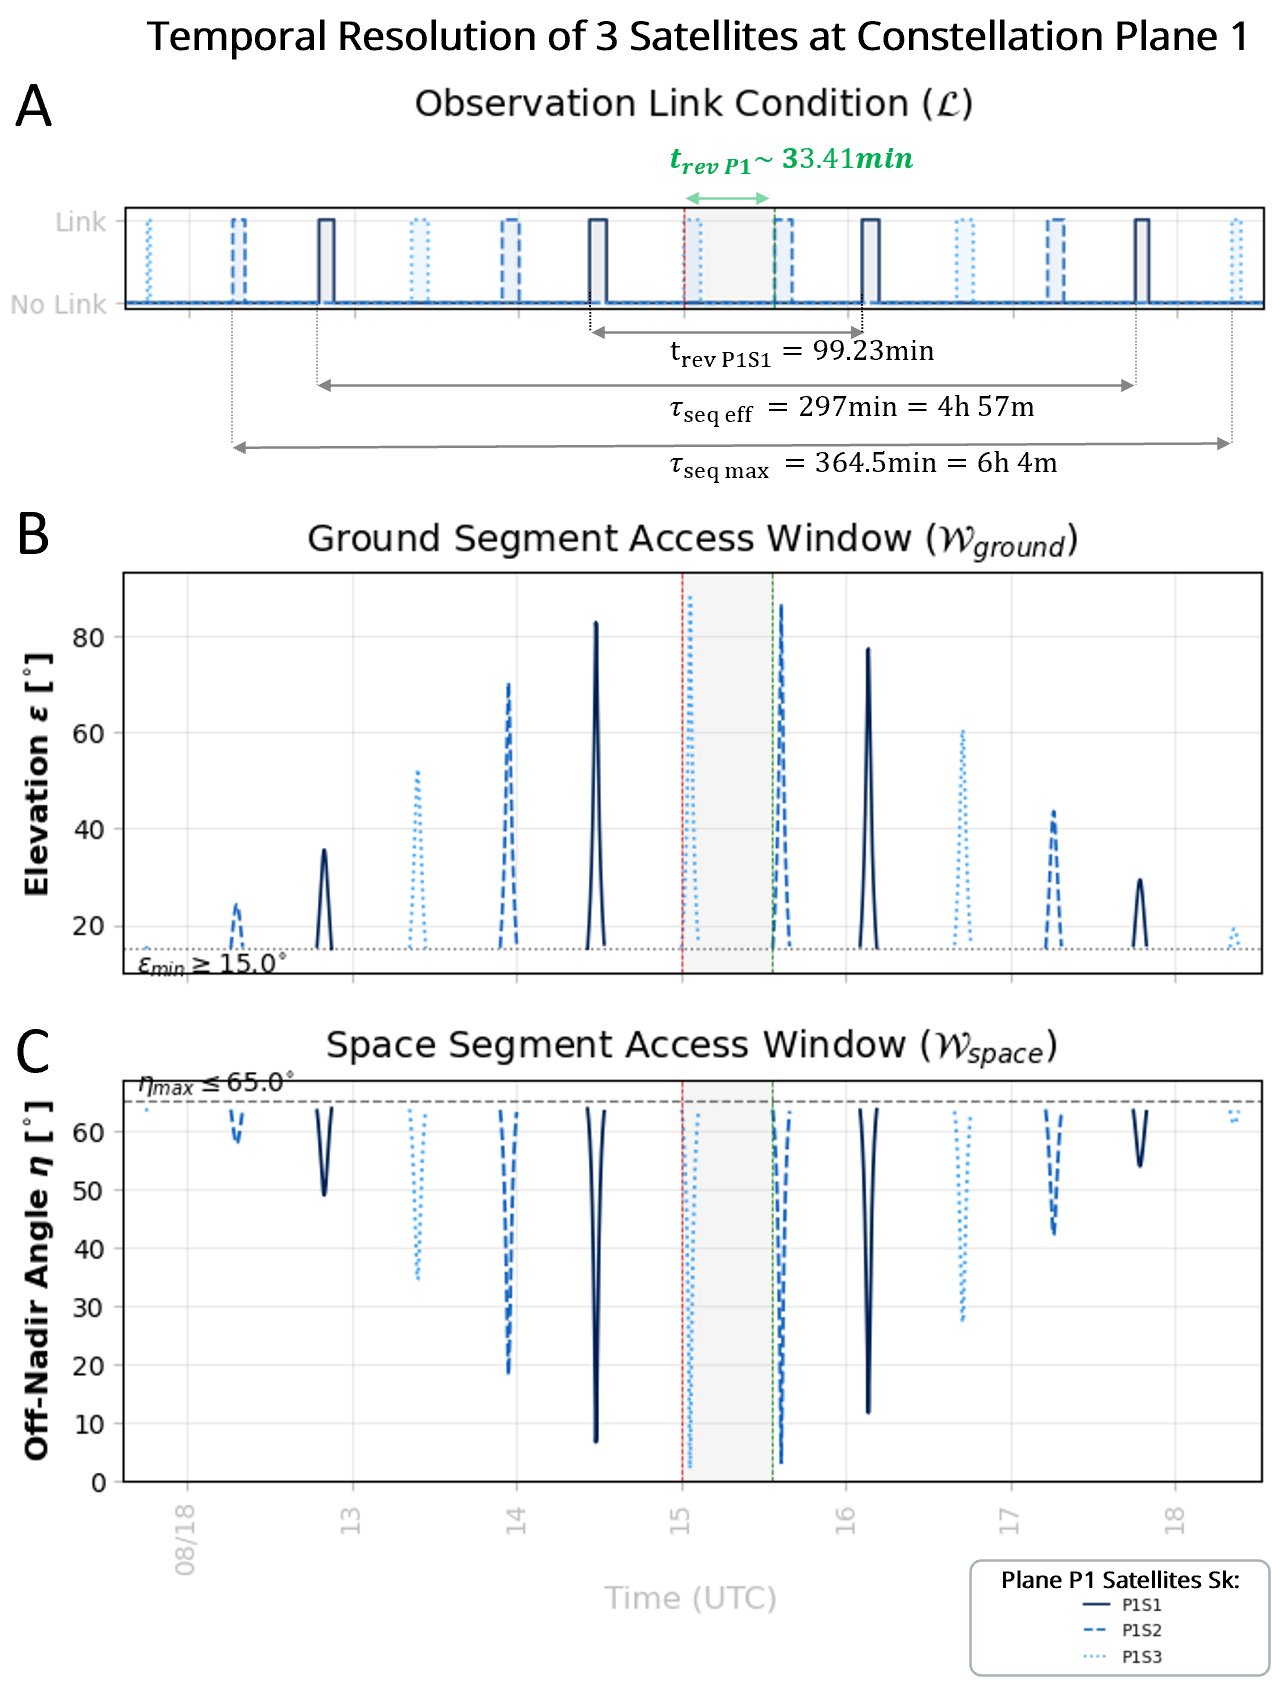
\includegraphics[width=1\linewidth]{images/temporal_resolution_observational_link_constellationP1S1.png}
    \caption{Observation-link analysis for Plane~1 with three co-planar satellites ($P_1S_1$--$P_1S_3$, $\Delta\nu = 120^{\circ}$) on the $\tau=15/1$ RGTO.  \textbf{(a)}~Combined observation-link condition.  \textbf{(b)}~Elevation profile ($t_{\mathrm{rev,P1}} \approx 33.4$\,min).  \textbf{(c)}~Off-nadir angle per pass.}
    \label{fig:temporal_res_P1S1}
\end{figure}

\begin{figure}
    \centering
    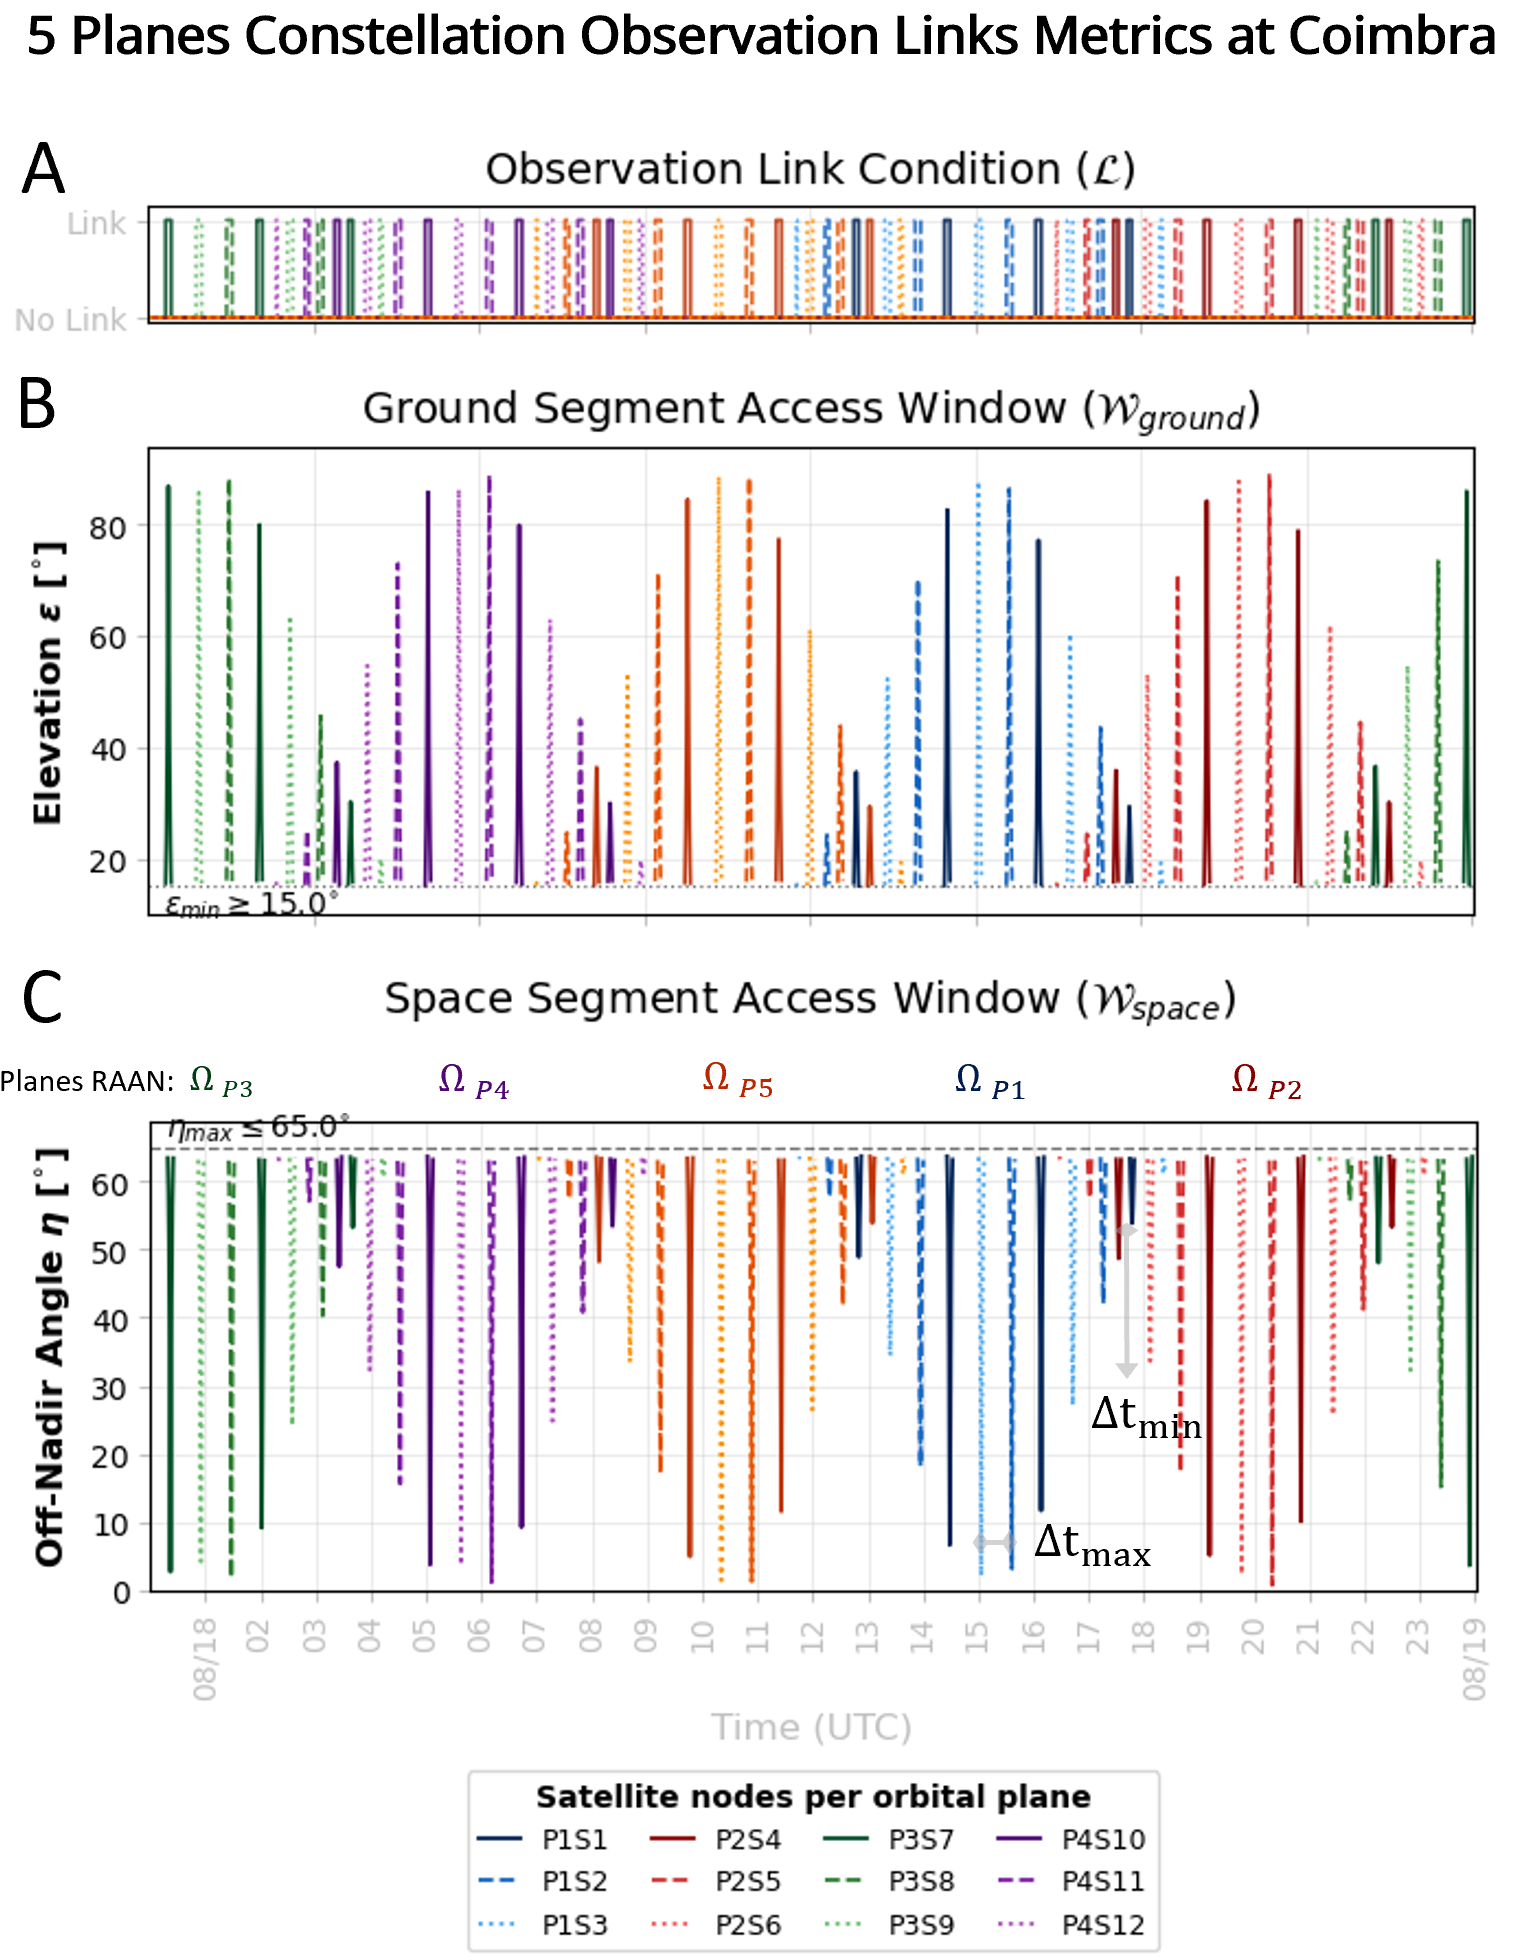
\includegraphics[width=1\linewidth]{images/5_planes_Constellation_Observation_Links_at_Coimbra.png}
    \caption{Observation links at Coimbra for the 5-plane Walker RGTO constellation $\mathcal{C}_{15/5/72}$ ($T_{\mathrm{seq,eff}} \approx 297$\,min, $\delta\Omega = 72^{\circ}$).  Each plane carries three satellites phased $120^{\circ}$ apart; the combined coverage spans the full day with $t_{\mathrm{rev}} \lesssim 33$\,min.}
    \label{fig:obs_links_5planes}
\end{figure}


\subsubsection{Conclusion: Baseline Constellation Parameters}
\label{sec:baseline_constellation_params}

The following parameters will be used in the next chapters to evaluate the performance of the baseline spacecraft cluster.
Table~\ref{tab:walker_c15} lists the RAAN and initial true anomaly for each of the 15~satellites in the baseline constellation $\mathcal{C}_{15/5/72}$.  All spacecraft share the RGTO seed orbit of Table~\ref{tab:rgto_parameters_coimbra} ($\tau=15/1$, $e=0.001$, $i=40.20329^{\circ}$, $\omega=0^{\circ}$), with $\Omega_{\mathrm{ref}}=100^{\circ}$ chosen to align $P_1S_1$ with the 18~August 15:00\,LT fire-peak pass over Coimbra.  This configuration, with $t_{\mathrm{rev}} \approx 33$\,min, is the closest Walker solution that satisfies the mission requirements $t_{\mathrm{rev}} \leq 30$\,min and GSD\,$< 6$\,m\,px$^{-1}$ throughout the full day over $\mathcal{D}_{\mathrm{core}}$, and is therefore adopted as the baseline constellation (\reqRef{R7}, \reqRef{R8}).

If sub-30-minute revisit is required, each plane can be further populated with four satellites phased $\Delta\nu = 90^{\circ}$, yielding $\mathcal{C}_{20/5/72}$ with $t_{\mathrm{rev}} \approx 25$\,min.  The full orbital-element tables for the baseline, the 4-plane candidate $\mathcal{C}_{12/4/90}$, and the high-cadence variant $\mathcal{C}_{20/5/72}$ are collected in Appendix~\ref{app:constellation_tables}, Table~\ref{tab:walker_constellations}.

\begin{table}[H]
\centering
\caption{\footnotesize{Baseline satellite parameter Walker RGTO constellation $\mathcal{C}_{15/5/72}$}}
\label{tab:walker_c15}
\smallskip
\footnotesize
\setlength{\tabcolsep}{4pt}
\begin{tabular}{c c r r}
\toprule
Plane & $S_k$ & $\Omega\;[^{\circ}]$ & $\nu_0\;[^{\circ}]$ \\
\midrule
\multirow{3}{*}{$P_1$} & $S_1$  & 100 &   0 \\
                        & $S_2$  & 100 & 120 \\
                        & $S_3$  & 100 & 240 \\
\midrule
\multirow{3}{*}{$P_2$} & $S_4$  & 172 &   0 \\
                        & $S_5$  & 172 & 120 \\
                        & $S_6$  & 172 & 240 \\
\midrule
\multirow{3}{*}{$P_3$} & $S_7$  & 244 &   0 \\
                        & $S_8$  & 244 & 120 \\
                        & $S_9$  & 244 & 240 \\
\midrule
\multirow{3}{*}{$P_4$} & $S_{10}$ & 316 &   0 \\
                        & $S_{11}$ & 316 & 120 \\
                        & $S_{12}$ & 316 & 240 \\
\midrule
\multirow{3}{*}{$P_5$} & $S_{13}$ &  28 &   0 \\
                        & $S_{14}$ &  28 & 120 \\
                        & $S_{15}$ &  28 & 240 \\
\bottomrule
\end{tabular}
\end{table}
